\documentclass[a4paper, 12pt]{article}
%%%%%%%%%%%%%%%%%%%%%%%%%%%%%%%%%%%%%%%%%%%%%%%%%%%%%%%%%%%%%%%%%%%%%%%%%%%%%%%
%                                Basic Packages                               %
%%%%%%%%%%%%%%%%%%%%%%%%%%%%%%%%%%%%%%%%%%%%%%%%%%%%%%%%%%%%%%%%%%%%%%%%%%%%%%%

% Gives us multiple colors.
\usepackage[usenames,dvipsnames,pdftex]{xcolor}
% Lets us style link colors.
\usepackage{hyperref}
% Lets us import images and graphics.
\usepackage{graphicx}
% Lets us use figures in floating environments.
\usepackage{float}
% Lets us create multiple columns.
\usepackage{multicol}
% Gives us better math syntax.
\usepackage{amsmath,amsfonts,mathtools,amsthm,amssymb}
% Lets us strikethrough text.
\usepackage{cancel}
% Lets us edit the caption of a figure.
\usepackage{caption}
% Lets us import pdf directly in our tex code.
\usepackage{pdfpages}
% Lets us do algorithm stuff.
\usepackage[ruled,vlined,linesnumbered]{algorithm2e}
% Use a smiley face for our qed symbol.
\usepackage{tikzsymbols}
% \usepackage{fullpage} %%smaller margins
\usepackage[shortlabels]{enumitem}

\setlist[enumerate]{font={\bfseries}} % global settings, for all lists

\usepackage{setspace}
\usepackage[margin=1in, headsep=12pt]{geometry}
\usepackage{wrapfig}
\usepackage{listings}
\usepackage{parskip}

\definecolor{codegreen}{rgb}{0,0.6,0}
\definecolor{codegray}{rgb}{0.5,0.5,0.5}
\definecolor{codepurple}{rgb}{0.58,0,0.82}
\definecolor{backcolour}{rgb}{0.95,0.95,0.95}

\lstdefinestyle{mystyle}{
    backgroundcolor=\color{backcolour},   
    commentstyle=\color{codegreen},
    keywordstyle=\color{magenta},
    numberstyle=\tiny\color{codegray},
    stringstyle=\color{codepurple},
    basicstyle=\ttfamily\footnotesize,
    breakatwhitespace=false,         
    breaklines=true,                 
    captionpos=b,                    
    keepspaces=true,                 
    numbers=left,                    
    numbersep=5pt,                  
    showspaces=false,                
    showstringspaces=false,
    showtabs=false,                  
    tabsize=2,
    numbers=none
}

\lstset{style=mystyle}
\def\class{article}


%%%%%%%%%%%%%%%%%%%%%%%%%%%%%%%%%%%%%%%%%%%%%%%%%%%%%%%%%%%%%%%%%%%%%%%%%%%%%%%
%                                Basic Settings                               %
%%%%%%%%%%%%%%%%%%%%%%%%%%%%%%%%%%%%%%%%%%%%%%%%%%%%%%%%%%%%%%%%%%%%%%%%%%%%%%%

%%%%%%%%%%%%%
%  Symbols  %
%%%%%%%%%%%%%

\let\implies\Rightarrow
\let\impliedby\Leftarrow
\let\iff\Leftrightarrow
\let\epsilon\varepsilon
%%%%%%%%%%%%
%  Tables  %
%%%%%%%%%%%%

\setlength{\tabcolsep}{5pt}
\renewcommand\arraystretch{1.5}

%%%%%%%%%%%%%%
%  SI Unitx  %
%%%%%%%%%%%%%%

\usepackage{siunitx}
\sisetup{locale = FR}

%%%%%%%%%%
%  TikZ  %
%%%%%%%%%%

\usepackage[framemethod=TikZ]{mdframed}
\usepackage{tikz}
\usepackage{tikz-cd}
\usepackage{tikzsymbols}

\usetikzlibrary{intersections, angles, quotes, calc, positioning}
\usetikzlibrary{arrows.meta}

\tikzset{
    force/.style={thick, {Circle[length=2pt]}-stealth, shorten <=-1pt}
}

%%%%%%%%%%%%%%%
%  PGF Plots  %
%%%%%%%%%%%%%%%

\usepackage{pgfplots}
\pgfplotsset{width=10cm, compat=newest}

%%%%%%%%%%%%%%%%%%%%%%%
%  Center Title Page  %
%%%%%%%%%%%%%%%%%%%%%%%

\usepackage{titling}
\renewcommand\maketitlehooka{\null\mbox{}\vfill}
\renewcommand\maketitlehookd{\vfill\null}

%%%%%%%%%%%%%%%%%%%%%%%%%%%%%%%%%%%%%%%%%%%%%%%%%%%%%%%
%  Create a grey background in the middle of the PDF  %
%%%%%%%%%%%%%%%%%%%%%%%%%%%%%%%%%%%%%%%%%%%%%%%%%%%%%%%

\usepackage{eso-pic}
\newcommand\definegraybackground{
    \definecolor{reallylightgray}{HTML}{FAFAFA}
    \AddToShipoutPicture{
        \ifthenelse{\isodd{\thepage}}{
            \AtPageLowerLeft{
                \put(\LenToUnit{\dimexpr\paperwidth-222pt},0){
                    \color{reallylightgray}\rule{222pt}{297mm}
                }
            }
        }
        {
            \AtPageLowerLeft{
                \color{reallylightgray}\rule{222pt}{297mm}
            }
        }
    }
}

%%%%%%%%%%%%%%%%%%%%%%%%
%  Modify Links Color  %
%%%%%%%%%%%%%%%%%%%%%%%%

\hypersetup{
    % Enable highlighting links.
    colorlinks,
    % Change the color of links to blue.
    urlcolor=blue,
    % Change the color of citations to black.
    citecolor={black},
    % Change the color of url's to blue with some black.
    linkcolor={blue!80!black}
}

%%%%%%%%%%%%%%%%%%
% Fix WrapFigure %
%%%%%%%%%%%%%%%%%%

\newcommand{\wrapfill}{\par\ifnum\value{WF@wrappedlines}>0
        \parskip=0pt
        \addtocounter{WF@wrappedlines}{-1}%
        \null\vspace{\arabic{WF@wrappedlines}\baselineskip}%
        \WFclear
    \fi}

%%%%%%%%%%%%%%%%%
% Multi Columns %
%%%%%%%%%%%%%%%%%

\let\multicolmulticols\multicols
\let\endmulticolmulticols\endmulticols

\RenewDocumentEnvironment{multicols}{mO{}}
{%
    \ifnum#1=1
        #2%
    \else % More than 1 column
        \multicolmulticols{#1}[#2]
    \fi
}
{%
    \ifnum#1=1
    \else % More than 1 column
        \endmulticolmulticols
    \fi
}

\newlength{\thickarrayrulewidth}
\setlength{\thickarrayrulewidth}{5\arrayrulewidth}


%%%%%%%%%%%%%%%%%%%%%%%%%%%%%%%%%%%%%%%%%%%%%%%%%%%%%%%%%%%%%%%%%%%%%%%%%%%%%%%
%                           School Specific Commands                          %
%%%%%%%%%%%%%%%%%%%%%%%%%%%%%%%%%%%%%%%%%%%%%%%%%%%%%%%%%%%%%%%%%%%%%%%%%%%%%%%

%%%%%%%%%%%%%%%%%%%%%%%%%%%
%  Initiate New Counters  %
%%%%%%%%%%%%%%%%%%%%%%%%%%%

\newcounter{lecturecounter}

%%%%%%%%%%%%%%%%%%%%%%%%%%
%  Helpful New Commands  %
%%%%%%%%%%%%%%%%%%%%%%%%%%

\makeatletter

\newcommand\resetcounters{
    % Reset the counters for subsection, subsubsection and the definition
    % all the custom environments.
    \setcounter{subsection}{0}
    \setcounter{subsubsection}{0}
    \setcounter{definition0}{0}
    \setcounter{paragraph}{0}
    \setcounter{theorem}{0}
    \setcounter{claim}{0}
    \setcounter{corollary}{0}
    \setcounter{proposition}{0}
    \setcounter{lemma}{0}
    \setcounter{exercise}{0}
    \setcounter{problem}{0}
    
    \setcounter{subparagraph}{0}
    % \@ifclasswith\class{nocolor}{
    %     \setcounter{definition}{0}
    % }{}
}

%%%%%%%%%%%%%%%%%%%%%
%  Lecture Command  %
%%%%%%%%%%%%%%%%%%%%%

\usepackage{xifthen}

% EXAMPLE:
% 1. \lecture{Oct 17 2022 Mon (08:46:48)}{Lecture Title}
% 2. \lecture[4]{Oct 17 2022 Mon (08:46:48)}{Lecture Title}
% 3. \lecture{Oct 17 2022 Mon (08:46:48)}{}
% 4. \lecture[4]{Oct 17 2022 Mon (08:46:48)}{}
% Parameters:
% 1. (Optional) lecture number.
% 2. Time and date of lecture.
% 3. Lecture Title.
\def\@lecture{}
\def\@lectitle{}
\def\@leccount{}
\newcommand\lecture[3]{
    \newpage

    % Check if user passed the lecture title or not.
    \def\@leccount{Lecture #1}
    \ifthenelse{\isempty{#3}}{
        \def\@lecture{Lecture #1}
        \def\@lectitle{Lecture #1}
    }{
        \def\@lecture{Lecture #1: #3}
        \def\@lectitle{#3}
    }

    \setcounter{section}{#1}
    \renewcommand\thesubsection{#1.\arabic{subsection}}
    
    \phantomsection
    \addcontentsline{toc}{section}{\@lecture}
    \resetcounters

    \begin{mdframed}
        \begin{center}
            \Large \textbf{\@leccount}
            
            \vspace*{0.2cm}
            
            \large \@lectitle
            
            
            \vspace*{0.2cm}

            \normalsize #2
        \end{center}
    \end{mdframed}

}

%%%%%%%%%%%%%%%%%%%%
%  Import Figures  %
%%%%%%%%%%%%%%%%%%%%

\usepackage{import}
\pdfminorversion=7

% EXAMPLE:
% 1. \incfig{limit-graph}
% 2. \incfig[0.4]{limit-graph}
% Parameters:
% 1. The figure name. It should be located in figures/NAME.tex_pdf.
% 2. (Optional) The width of the figure. Example: 0.5, 0.35.
\newcommand\incfig[2][1]{%
    \def\svgwidth{#1\columnwidth}
    \import{./figures/}{#2.pdf_tex}
}

\begingroup\expandafter\expandafter\expandafter\endgroup
\expandafter\ifx\csname pdfsuppresswarningpagegroup\endcsname\relax
\else
    \pdfsuppresswarningpagegroup=1\relax
\fi

%%%%%%%%%%%%%%%%%
% Fancy Headers %
%%%%%%%%%%%%%%%%%

\usepackage{fancyhdr}

% Force a new page.
\newcommand\forcenewpage{\clearpage\mbox{~}\clearpage\newpage}

% This command makes it easier to manage my headers and footers.
\newcommand\createintro{
    % Use roman page numbers (e.g. i, v, vi, x, ...)
    \pagenumbering{roman}

    % Display the page style.
    \maketitle
    % Make the title pagestyle empty, meaning no fancy headers and footers.
    \thispagestyle{empty}
    % Create a newpage.
    \newpage

    % Input the intro.tex page if it exists.
    \IfFileExists{intro.tex}{ % If the intro.tex file exists.
        % Input the intro.tex file.
        \textbf{Course}: MATH 16300: Honors Calculus III

\textbf{Section}: 43

\textbf{Professor}: Minjae Park

\textbf{At}: The University of Chicago

\textbf{Quarter}: Spring 2023

\textbf{Course materials}: Calculus by Spivak (4th Edition), Calculus On Manifolds by Spivak

\vspace{1cm}
\textbf{Disclaimer}: This document will inevitably contain some mistakes, both simple typos and serious logical and mathematical errors. Take what you read with a grain of salt as it is made by an undergraduate student going through the learning process himself. If you do find any error, I would really appreciate it if you can let me know by email at \href{mailto:conghungletran@gmail.com}{conghungletran@gmail.com}.

        % Make the pagestyle fancy for the intro.tex page.
        \pagestyle{fancy}

        % Remove the line for the header.
        \renewcommand\headrulewidth{0pt}

        % Remove all header stuff.
        \fancyhead{}

        % Add stuff for the footer in the center.
        % \fancyfoot[C]{
        %   \textit{For more notes like this, visit
        %   \href{\linktootherpages}{\shortlinkname}}. \\
        %   \vspace{0.1cm}
        %   \hrule
        %   \vspace{0.1cm}
        %   \@author, \\
        %   \term: \academicyear, \\
        %   Last Update: \@date, \\
        %   \faculty
        % }

        \newpage
    }{ % If the intro.tex file doesn't exist.
        % Force a \newpageage.
        % \forcenewpage
        \newpage
    }

    % Remove the center stuff we did above, and replace it with just the page
    % number, which is still in roman numerals.
    \fancyfoot[C]{\thepage}
    % Add the table of contents.
    \tableofcontents
    % Force a new page.
    \newpage

    % Move the page numberings back to arabic, from roman numerals.
    \pagenumbering{arabic}
    % Set the page number to 1.
    \setcounter{page}{1}

    % Add the header line back.
    \renewcommand\headrulewidth{0.4pt}
    % In the top right, add the lecture title.
    \fancyhead[R]{\footnotesize \@lecture}
    % In the top left, add the author name.
    \fancyhead[L]{\footnotesize \@author}
    % In the bottom center, add the page.
    \fancyfoot[C]{\thepage}
    % Add a nice gray background in the middle of all the upcoming pages.
    % \definegraybackground
}

\makeatother


%%%%%%%%%%%%%%%%%%%%%%%%%%%%%%%%%%%%%%%%%%%%%%%%%%%%%%%%%%%%%%%%%%%%%%%%%%%%%%%
%                               Custom Commands                               %
%%%%%%%%%%%%%%%%%%%%%%%%%%%%%%%%%%%%%%%%%%%%%%%%%%%%%%%%%%%%%%%%%%%%%%%%%%%%%%%

%%%%%%%%%%%%
%  Circle  %
%%%%%%%%%%%%

\newcommand*\circled[1]{\tikz[baseline= (char.base)]{
        \node[shape=circle,draw,inner sep=1pt] (char) {#1};}
}

%%%%%%%%%%%%%%%%%%%
%  Todo Commands  %
%%%%%%%%%%%%%%%%%%%

% \usepackage{xargs}
% \usepackage[colorinlistoftodos]{todonotes}

% \makeatletter

% \@ifclasswith\class{working}{
%     \newcommandx\unsure[2][1=]{\todo[linecolor=red,backgroundcolor=red!25,bordercolor=red,#1]{#2}}
%     \newcommandx\change[2][1=]{\todo[linecolor=blue,backgroundcolor=blue!25,bordercolor=blue,#1]{#2}}
%     \newcommandx\info[2][1=]{\todo[linecolor=OliveGreen,backgroundcolor=OliveGreen!25,bordercolor=OliveGreen,#1]{#2}}
%     \newcommandx\improvement[2][1=]{\todo[linecolor=Plum,backgroundcolor=Plum!25,bordercolor=Plum,#1]{#2}}

%     \newcommand\listnotes{
%         \newpage
%         \listoftodos[Notes]
%     }
% }{
%     \newcommandx\unsure[2][1=]{}
%     \newcommandx\change[2][1=]{}
%     \newcommandx\info[2][1=]{}
%     \newcommandx\improvement[2][1=]{}

%     \newcommand\listnotes{}
% }

% \makeatother

%%%%%%%%%%%%%
%  Correct  %
%%%%%%%%%%%%%

% EXAMPLE:
% 1. \correct{INCORRECT}{CORRECT}
% Parameters:
% 1. The incorrect statement.
% 2. The correct statement.
\definecolor{correct}{HTML}{009900}
\newcommand\correct[2]{{\color{red}{#1 }}\ensuremath{\to}{\color{correct}{ #2}}}


%%%%%%%%%%%%%%%%%%%%%%%%%%%%%%%%%%%%%%%%%%%%%%%%%%%%%%%%%%%%%%%%%%%%%%%%%%%%%%%
%                                 Environments                                %
%%%%%%%%%%%%%%%%%%%%%%%%%%%%%%%%%%%%%%%%%%%%%%%%%%%%%%%%%%%%%%%%%%%%%%%%%%%%%%%

\usepackage{varwidth}
\usepackage{thmtools}
\usepackage[most,many,breakable]{tcolorbox}

\tcbuselibrary{theorems,skins,hooks}
\usetikzlibrary{arrows,calc,shadows.blur}

%%%%%%%%%%%%%%%%%%%
%  Define Colors  %
%%%%%%%%%%%%%%%%%%%

% color prototype
% \definecolor{color}{RGB}{45, 111, 177}

% ESSENTIALS: 
\definecolor{myred}{HTML}{c74540}
\definecolor{myblue}{HTML}{072b85}
\definecolor{mygreen}{HTML}{388c46}
\definecolor{myblack}{HTML}{000000}

\colorlet{definition_color}{myred}

\colorlet{theorem_color}{myblue}
\colorlet{lemma_color}{myblue}
\colorlet{prop_color}{myblue}
\colorlet{corollary_color}{myblue}
\colorlet{claim_color}{myblue}

\colorlet{proof_color}{myblack}
\colorlet{example_color}{myblack}
\colorlet{exercise_color}{myblack}

% MISCS: 
%%%%%%%%%%%%%%%%%%%%%%%%%%%%%%%%%%%%%%%%%%%%%%%%%%%%%%%%%
%  Create Environments Styles Based on Given Parameter  %
%%%%%%%%%%%%%%%%%%%%%%%%%%%%%%%%%%%%%%%%%%%%%%%%%%%%%%%%%

% \mdfsetup{skipabove=1em,skipbelow=0em}

%%%%%%%%%%%%%%%%%%%%%%
%  Helpful Commands  %
%%%%%%%%%%%%%%%%%%%%%%

% EXAMPLE:
% 1. \createnewtheoremstyle{thmdefinitionbox}{}{}
% 2. \createnewtheoremstyle{thmtheorembox}{}{}
% 3. \createnewtheoremstyle{thmproofbox}{qed=\qedsymbol}{
%       rightline=false, topline=false, bottomline=false
%    }
% Parameters:
% 1. Theorem name.
% 2. Any extra parameters to pass directly to declaretheoremstyle.
% 3. Any extra parameters to pass directly to mdframed.
\newcommand\createnewtheoremstyle[3]{
    \declaretheoremstyle[
        headfont=\bfseries\sffamily, bodyfont=\normalfont, #2,
        mdframed={
                #3,
            },
    ]{#1}
}

% EXAMPLE:
% 1. \createnewcoloredtheoremstyle{thmdefinitionbox}{definition}{}{}
% 2. \createnewcoloredtheoremstyle{thmexamplebox}{example}{}{
%       rightline=true, leftline=true, topline=true, bottomline=true
%     }
% 3. \createnewcoloredtheoremstyle{thmproofbox}{proof}{qed=\qedsymbol}{backgroundcolor=white}
% Parameters:
% 1. Theorem name.
% 2. Color of theorem.
% 3. Any extra parameters to pass directly to declaretheoremstyle.
% 4. Any extra parameters to pass directly to mdframed.

% change backgroundcolor to #2!5 if user wants a colored backdrop to theorem environments. It's a cool color theme, but there's too much going on in the page.
\newcommand\createnewcoloredtheoremstyle[4]{
    \declaretheoremstyle[
        headfont=\bfseries\sffamily\color{#2},
        bodyfont=\normalfont,
        headpunct=,
        headformat = \NAME~\NUMBER\NOTE \hfill\smallskip\linebreak,
        #3,
        mdframed={
                outerlinewidth=0.75pt,
                rightline=false,
                leftline=false,
                topline=false,
                bottomline=false,
                backgroundcolor=white,
                skipabove = 5pt,
                skipbelow = 0pt,
                linecolor=#2,
                innertopmargin = 0pt,
                innerbottommargin = 0pt,
                innerrightmargin = 4pt,
                innerleftmargin= 6pt,
                leftmargin = -6pt,
                #4,
            },
    ]{#1}
}



%%%%%%%%%%%%%%%%%%%%%%%%%%%%%%%%%%%
%  Create the Environment Styles  %
%%%%%%%%%%%%%%%%%%%%%%%%%%%%%%%%%%%

\makeatletter
\@ifclasswith\class{nocolor}{
    % Environments without color.

    % ESSENTIALS:
    \createnewtheoremstyle{thmdefinitionbox}{}{}
    \createnewtheoremstyle{thmtheorembox}{}{}
    \createnewtheoremstyle{thmproofbox}{qed=\qedsymbol}{}
    \createnewtheoremstyle{thmcorollarybox}{}{}
    \createnewtheoremstyle{thmlemmabox}{}{}
    \createnewtheoremstyle{thmclaimbox}{}{}
    \createnewtheoremstyle{thmexamplebox}{}{}

    % MISCS: 
    \createnewtheoremstyle{thmpropbox}{}{}
    \createnewtheoremstyle{thmexercisebox}{}{}
    \createnewtheoremstyle{thmexplanationbox}{}{}
    \createnewtheoremstyle{thmremarkbox}{}{}
    
    % STYLIZED MORE BELOW
    \createnewtheoremstyle{thmquestionbox}{}{}
    \createnewtheoremstyle{thmsolutionbox}{qed=\qedsymbol}{}
}{
    % Environments with color.

    % ESSENTIALS: definition, theorem, proof, corollary, lemma, claim, example
    \createnewcoloredtheoremstyle{thmdefinitionbox}{definition_color}{}{leftline=false}
    \createnewcoloredtheoremstyle{thmtheorembox}{theorem_color}{}{leftline=false}
    \createnewcoloredtheoremstyle{thmproofbox}{proof_color}{qed=\qedsymbol}{}
    \createnewcoloredtheoremstyle{thmcorollarybox}{corollary_color}{}{leftline=false}
    \createnewcoloredtheoremstyle{thmlemmabox}{lemma_color}{}{leftline=false}
    \createnewcoloredtheoremstyle{thmpropbox}{prop_color}{}{leftline=false}
    \createnewcoloredtheoremstyle{thmclaimbox}{claim_color}{}{leftline=false}
    \createnewcoloredtheoremstyle{thmexamplebox}{example_color}{}{}
    \createnewcoloredtheoremstyle{thmexplanationbox}{example_color}{qed=\qedsymbol}{}
    \createnewcoloredtheoremstyle{thmremarkbox}{theorem_color}{}{}

    \createnewcoloredtheoremstyle{thmmiscbox}{black}{}{}

    \createnewcoloredtheoremstyle{thmexercisebox}{exercise_color}{}{}
    \createnewcoloredtheoremstyle{thmproblembox}{theorem_color}{}{leftline=false}
    \createnewcoloredtheoremstyle{thmsolutionbox}{mygreen}{qed=\qedsymbol}{}
}
\makeatother

%%%%%%%%%%%%%%%%%%%%%%%%%%%%%
%  Create the Environments  %
%%%%%%%%%%%%%%%%%%%%%%%%%%%%%
\declaretheorem[numberwithin=section, style=thmdefinitionbox,     name=Definition]{definition}
\declaretheorem[numberwithin=section, style=thmtheorembox,     name=Theorem]{theorem}
\declaretheorem[numbered=no,          style=thmexamplebox,     name=Example]{example}
\declaretheorem[numberwithin=section, style=thmtheorembox,       name=Claim]{claim}
\declaretheorem[numberwithin=section, style=thmcorollarybox,   name=Corollary]{corollary}
\declaretheorem[numberwithin=section, style=thmpropbox,        name=Proposition]{proposition}
\declaretheorem[numberwithin=section, style=thmlemmabox,       name=Lemma]{lemma}
\declaretheorem[numberwithin=section, style=thmexercisebox,    name=Exercise]{exercise}
\declaretheorem[numbered=no,          style=thmproofbox,       name=Proof]{proof0}
\declaretheorem[numbered=no,          style=thmexplanationbox, name=Explanation]{explanation}
\declaretheorem[numbered=no,          style=thmsolutionbox,    name=Solution]{solution}
\declaretheorem[numberwithin=section,          style=thmproblembox,     name=Problem]{problem}
\declaretheorem[numbered=no,          style=thmmiscbox,    name=Intuition]{intuition}
\declaretheorem[numbered=no,          style=thmmiscbox,    name=Goal]{goal}
\declaretheorem[numbered=no,          style=thmmiscbox,    name=Recall]{recall}
\declaretheorem[numbered=no,          style=thmmiscbox,    name=Motivation]{motivation}
\declaretheorem[numbered=no,          style=thmmiscbox,    name=Remark]{remark}
\declaretheorem[numbered=no,          style=thmmiscbox,    name=Observe]{observe}
\declaretheorem[numbered=no,          style=thmmiscbox,    name=Question]{question}


%%%%%%%%%%%%%%%%%%%%%%%%%%%%
%  Edit Proof Environment  %
%%%%%%%%%%%%%%%%%%%%%%%%%%%%

\renewenvironment{proof}[2][\proofname]{
    % \vspace{-12pt}
    \begin{proof0} [#2]
        }{\end{proof0}}

\theoremstyle{definition}

\newtheorem*{notation}{Notation}
\newtheorem*{previouslyseen}{As previously seen}
\newtheorem*{property}{Property}
% \newtheorem*{intuition}{Intuition}
% \newtheorem*{goal}{Goal}
% \newtheorem*{recall}{Recall}
% \newtheorem*{motivation}{Motivation}
% \newtheorem*{remark}{Remark}
% \newtheorem*{observe}{Observe}

\author{Hung C. Le Tran}


%%%% MATH SHORTHANDS %%%%
%% blackboard bold math capitals
\DeclareMathOperator*{\esssup}{ess\,sup}
\DeclareMathOperator*{\Hom}{Hom}
\newcommand{\bbf}{\mathbb{F}}
\newcommand{\bbn}{\mathbb{N}}
\newcommand{\bbq}{\mathbb{Q}}
\newcommand{\bbr}{\mathbb{R}}
\newcommand{\bbz}{\mathbb{Z}}
\newcommand{\bbc}{\mathbb{C}}
\newcommand{\bbk}{\mathbb{K}}
\newcommand{\bbm}{\mathbb{M}}
\newcommand{\bbp}{\mathbb{P}}
\newcommand{\bbe}{\mathbb{E}}

\newcommand{\bfw}{\mathbf{w}}
\newcommand{\bfx}{\mathbf{x}}
\newcommand{\bfX}{\mathbf{X}}
\newcommand{\bfy}{\mathbf{y}}
\newcommand{\bfyhat}{\mathbf{\hat{y}}}

\newcommand{\calb}{\mathcal{B}}
\newcommand{\calf}{\mathcal{F}}
\newcommand{\calt}{\mathcal{T}}
\newcommand{\call}{\mathcal{L}}
\renewcommand{\phi}{\varphi}

% Universal Math Shortcuts
\newcommand{\st}{\hspace*{2pt}\text{s.t.}\hspace*{2pt}}
\newcommand{\pffwd}{\hspace*{2pt}\fbox{\(\Rightarrow\)}\hspace*{10pt}}
\newcommand{\pfbwd}{\hspace*{2pt}\fbox{\(\Leftarrow\)}\hspace*{10pt}}
\newcommand{\contra}{\ensuremath{\Rightarrow\Leftarrow}}
\newcommand{\cvgn}{\xrightarrow{n \to \infty}}
\newcommand{\cvgj}{\xrightarrow{j \to \infty}}

\newcommand{\im}{\mathrm{im}}
\newcommand{\innerproduct}[2]{\langle #1, #2 \rangle}
\newcommand*{\conj}[1]{\overline{#1}}

% https://tex.stackexchange.com/questions/438612/space-between-exists-and-forall
% https://tex.stackexchange.com/questions/22798/nice-looking-empty-set
\let\oldforall\forall
\renewcommand{\forall}{\;\oldforall\; }
\let\oldexist\exists
\renewcommand{\exists}{\;\oldexist\; }
\newcommand\existu{\;\oldexist!\: }
\let\oldemptyset\emptyset
\let\emptyset\varnothing


\renewcommand{\_}[1]{\underline{#1}}
\DeclarePairedDelimiter{\abs}{\lvert}{\rvert}
\DeclarePairedDelimiter{\norm}{\lVert}{\rVert}
\DeclarePairedDelimiter\ceil{\lceil}{\rceil}
\DeclarePairedDelimiter\floor{\lfloor}{\rfloor}
\setlength\parindent{0pt}
\setlength{\headheight}{12.0pt}
\addtolength{\topmargin}{-12.0pt}


% Default skipping, change if you want more spacing
% \thinmuskip=3mu
% \medmuskip=4mu plus 2mu minus 4mu
% \thickmuskip=5mu plus 5mu

% \DeclareMathOperator{\ext}{ext}
% \DeclareMathOperator{\bridge}{bridge}
\title{MATH 20700: Honors Analysis in Rn I \\ \large Problem Set 3}
\date{15 Oct 2023}
\author{Hung Le Tran}
\begin{document}
\maketitle
\setcounter{section}{3}
\textbf{Textbook: Pugh's Real Mathematical Analysis}

\textit{Collaborators: Lucio}
\begin{problem} [2.118*]
The implications of compactness are frequently equivalent to it. Prove
\begin{enumerate} [(a)]
    \item If every continuous function $f: M \to \bbr$ is bounded then $M$ is compact.
    \item If every continuous bounded function $f: M \to \bbr$ achieves a maximum or minimum then $M$ is compact.
    \item If every continuous function $f: M \to \bbr$ has compact range $fM$ then $M$ is compact.
    \item If every nested decreasing sequence of nonempty closed subsets of $M$ has nonempty intersection then $M$ is compact.
\end{enumerate}

Toegether with Theorems 63 and 65, (a)-(d) give seven equivalent definitions of compactness. [Hint: Reason contrapositively. If $M$ is not compact then it contains a sequence $\{p_n\}$ that has no convergent subsequence. It is fair to assume that the points $p_n$ are distinct. Find radii $r_n > 0$ such that the neighborhoods $M_{r_n}(p_n)$ are disjoint and no sequence $q_n \in M_{r_n}(p_n)$ has a convergent subsequence. Using the metric define a function $f_n: M_{r_n} (p_n) \to \bbr$ with a spike at $p_n$, such as \[
            f_n(x) = \frac{r_n - d(x, p_n)}{a_n + d(x, p_n)}
        \]
        where $a_n > 0$. Set $f(x) = f_n(x)$ if $x \in M_{r_n}(p_n)$, and $f(x) = 0$ if $x$ belongs to no $M_{r_n}(p_n)$. Show that $f$ is continuous. With the right choice of $a_n$ show that $f$ is unbounded. With a different choice of $a_n$, it is bounded but achieves no maximum, and so on.]
\end{problem}
\begin{solution}
    \textbf{(a)} Suppose $M$ is not compact. Then there exists sequence $\{p_n\} \subseteq M$ such that it has no convergent subsequence.

    We first prove that there exists radii $r_n > 0$ such that $B(x_n, r_n)$ are pairwise disjoint.

    Let $d_n = \inf_{i \neq n}\{d(p_n, p_i)\}$ and set $r_n = d_n/3$, which requires to show that $d_n \neq 0$.

    Suppose that it is. Then \[
        \forall \epsilon > 0, \exists N_\epsilon \:\text{such that}\: d(p_n, p_{N_\epsilon}) < \epsilon
    \]
    We derive a contradiction by constructing a converging subsequence of $\{p_n\}$.

    Choose $\epsilon_1 = 1$, then there exists $N_1$ such that $d(p_n, p_{N_1}) < 1$.

    Choose $\epsilon_2 = \min\{\epsilon_1 /2, \min_{j \leq N_1}\{d(p_n, p_j)\}/2\}$, then there exists $N_2$ such that

    $d(p_n, p_{N_2}) < \epsilon_2$. Note that $N_2 > N_1$ due to the construction of $\epsilon_2$, and that $\epsilon_2 \leq 1/2$.

    Continue constructing this way, since $N_{j+1} > N_{j}$, we get a subsequence $\{p_{N_j}\}_{j \in \bbn}$ that satisfies \[
        d(p_{N_j}, p_n) < \epsilon_j \leq 1/2^j
    \]
    which therefore converges to $p_n$. \contra

    It follows that $d_n > 0$. Coming back, if we set $r_n = d_n/3$ then \[
        d(p_n, p_m) > d(p_n, p_m)/3 + d(p_m, p_n)/3 \leq r_n + r_m
    \]
    so the balls $B(p_n, r_n)$ and $B(p_m, r_m)$ are disjoint for all $m \neq n$.

    A fact that we won't rigorously prove is that there can't be any sequence $q_n \in B(p_n, r_n)$ that has a convergent subsequence. Simply put, if there exists a convergent subsequence of $\{q_n\}$, since $r_n \cvgn 0$, there ought to exist a corresponding subsequence of $\{p_n\}$ too.

    Then, define \[
        f_n(x) = \frac{r_n - d(x, p_n)}{a_n + d(x, p_n)}
    \]
    on $B(p_n, r_n)$, for some $a_n > 0$. We define $f(x) = f_n(x)$ on $B(p_n, r_n)$ and 0 elsewhere.

    We now prove that $f$ is \textbf{continuous}. Let $R = M \backslash \bigsqcup_{n \in \bbn} B(p_n, r_n)$.

    Since $d$ is continuous, $f_n(x)$ is continuous too, so $f$ is continuous on $B(p_n, r_n)$. Take $y \in \partial B(p_n, r_n)$ then $f(y) = 0$. And if $y_n \in M \cvgn y$, $f(y_n) \cvgn 0$ too, since $d$ is continuous and $f \equiv 0$ on $R$. It follows that $f$ is continuous on $M$.

    So far we have not specified which $a_n$; $f$ is continuous for all $\{a_n\}_{n \in \bbn} \subset \bbr^+$. For each of the following sections we choose $a_n$ so as to bring about a contradiction, to then conclude that $M$ has to be compact.

    \textbf{(a)} Choose $a_n = \frac{r_n}{n} \implies f(p_n) = n$ which is unbounded. \contra

    \textbf{(b)} Choose $a_n = \frac{r_n}{2 - \frac{1}{n}}$ then (denote $d(x, p_n)$ as $d$)
    \begin{align*}
        f_n(x) & = \frac{r_n - d}{a_n + d}                                              \\
               & = \frac{r_n + a_n}{a_n + d} - 1                                        \\
               & \leq \frac{r_n + a_n}{a_n} - 1 = \frac{r_n}{a_n} = 2 - \frac{1}{n} < 2
    \end{align*}
    is therefore bounded but never achieves its maximum.

    Because if it does, it will be at some point $p_n$ (not other points in $M$), but $f(p_n) = 2 - \frac{1}{n}$. \contra

    \textbf{(c)} Choose $a_n = \frac{r_n}{n} \implies f(p_n) = n \implies \bbn \subset fM$. It follows that $fM$ is unbounded, and therefore can't be compact. \contra

    \textbf{(d)} Choose the same $a_n$. Define $K_n = \bbn \backslash \{k \in \bbn \mid k \leq n\}$, i.e., the natural numbers from $n$ onwards. Since for all $n$, there exists $f_n(p_n) = n$ so $f^{Pre}(K_n)$ is nonempty.

    $f$ is continuous and $K_n$ is closed in $\bbr$, so $f^{Pre}(K_n)$ is also closed.

    Since $K_1 \subset K_2 \subset K_3 \dots \implies f^{Pre}(K_1) \subset f^{Pre}(K_2) \subset \dots$ is a nested decreasing sequence.

    WTS $\bigcap_{n \in \bbn}f^{Pre}(K_n) = \emptyset$. Suppose there exists $y \in \bigcap_{n \in \bbn}f^{Pre}(K_n)$.

    Then $y \in f^{Pre}(K_n) \forall n$. It follows that $f(y) \in K_n \forall n \in \bbn$. Specifically $f(y) \in K_1 \implies f(y) \in \bbn, f(y) \geq 2$. Thus $f(y) = m \in \bbn, m \geq 2$.

    But then $f(y) \not \in K_m$. \contra
\end{solution}

\begin{problem} [2.152]
Write jingles at least as good as the following. Pay attention to the meter as well as the rhyme.

\begin{center}
    When a set in the plane

    is closed and bounded

    you can always draw

    a curve around it.
\end{center}
\end{problem}
\begin{solution}
\end{solution}

\begin{problem} [3.17]
Define $\frake: \bbr \to \bbr$ by \[
    \frake(x) = \begin{cases}
        e^{-1/x} & \:\text{if}\: x > 0    \\
        0        & \:\text{if}\: x \leq 0
    \end{cases}
\]
\begin{enumerate} [(a)]
    \item Prove that $\frake$ is smooth; that is, $\frake$ has derivatives of all orders at all points $x$. [Hint: L'Hopital and induction. Feel free to use the standard differentiation formulas about $e^x$ from calculus.]
    \item Is $\frake$ analytic?
    \item \textit{[Omitted in pset]} The bump function \[
              \beta(x) = e^2\frake(1-x)\frake(x+1)
          \]
    \item For $|x| < 1$, show that the bump function \[
              \beta(x) = e^{2x^2/(x^2-1)}
          \]
          Bump functions have wide use in smooth function theory and differential topology. The graph of $\beta$ looks like a bump.
\end{enumerate}
\end{problem}
\begin{solution}
    \textbf{(a)} Let $P_r$ be the proposition that there exists $r-$th order derivative of $\frake$ on $\bbr$, namely:
    \[
        \frake^{(r)}(x) = \begin{cases}
            A(1/x)e^{-1/x} & \:\text{for}\: x > 0    \\
            0              & \:\text{for}\: x \leq 0
        \end{cases}
    \]
    where $A(1/x)$ is a polynomial in $1/x$.

    \textbf{Base case:} $r = 1$.

    When $x < 0$, $\frake'(x) = 0$.

    When $x > 0$, $\frake'(x) = x^{-2} e^{-1/x}$.

    Let's consider $x = 0$ and estimate:
    \begin{align*}
        \lim_{x \to 0+} \frac{e^{-1/x} - 0}{x - 0} & = \lim_{x \to 0+} \frac{1/x}{e^{1/x}} \\
                                                   & =\lim_{p \to \infty}\frac{p}{e^p} = 0
    \end{align*}
    since $e^p$ grows faster than any polynomial $p^m$. Meanwhile, it's trivial that \[
        \lim_{x \to 0-} \frac{\frake(x) - 0}{x - 0 } = 0
    \]
    so $\frake'(0) = 0$. Therefore \[
        \frake'(x) = \begin{cases}
            x^{-2} e^{-1/x} & \:\text{for}\: x > 0    \\
            0               & \:\text{for}\: x \leq 0
        \end{cases}
    \]

    $P_1$ is therefore true.

    \textbf{Inductive case:} Suppose that $P_k$ is true:
    \[
        \frake^{(k)}(x) = \begin{cases}
            A(x)e^{-1/x} & \:\text{for}\: x > 0    \\
            0            & \:\text{for}\: x \leq 0
        \end{cases}
    \]
    We want to show that $P_{k+1}$ is also true.

    Then for $x > 0$,
    \begin{align*}
        \frake^{(k+1)}(x) & = A'(1/x)e^{-1/x} + A(x)[x^{-2}e^{-1/x}] \\
                          & = B(x)e^{-1/x}
    \end{align*}
    since if $A(1/x) = \sum_{j = 0}^{l}a_jx^{-j}$ then \[
        A'(1/x) = \sum_{j=0}^{l}(-j)a_jx^{-j-1}
    \]
    is another polynomial in $1/x$.

    For $x < 0$, it's trivial that $\frake^{k+1}(x) = 0$.

    Consider when $x = 0$, estimate:
    \begin{align*}
        \lim_{x \to 0+} \frac{\frake^{(k)}(x) - 0}{x - 0} & = \lim_{x \to 0+} \frac{A(1/x)e^{-1/x}}{x} \\
                                                          & =\lim_{p \to \infty}\frac{pA(p)}{e^p} = 0
    \end{align*}
    since $e^p$ grows faster than polynomial $pA(p)$.

    The limit from 0- is also 0, so we can conclude \[
        \frake^{(k+1)}(x) = \begin{cases}
            B(1/x)e^{-1/x} & \:\text{for}\: x > 0    \\
            0              & \:\text{for}\: x \leq 0
        \end{cases}
    \]
    so $P_{k+1}$ is also true.

    \textbf{Conclusion:} By mathematical induction, $P_n$ is true for all $n \in \bbn$. $\frake$ therefore has derivatives of all orders on $\bbr$. \qed

    \textbf{(b)} It is not analytic around $x = 0$.

    Suppose that it is, then there exists $\delta > 0$ such that if $|h| < \delta$ then \[
        \sum_{r = 0}^{\infty}\frac{\frake^r(0)}{r!}h^r = f(h)
    \]
    (the series converges to $f(h)$).

    But $LHS = 0$ and $f(h) > 0 \forall h > 0$. \contra \qed

    \textbf{(d)} For $|x| < 1$, we have $1-x > 0, x + 1 > 0$. Therefore \begin{align*}
        e^2\frake(1-x)\frake(x+1) & = e^2 e^{-1/(1-x)} e^{-1/(x+1)}         \\
                                  & = e^{2 - \frac{1}{1-x} - \frac{1}{x+1}} \\
                                  & = e^{2x^2/(x^2-1)}
    \end{align*}
\end{solution}

\begin{problem} [3.19]
Recall that the oscillation of an arbitrary function $f: [a, b] \to \bbr$ at $x$ is \[
    \rmosc_x f = \limsup_{t \to x}f(t) - \liminf_{t \to x} f(t)
\]
In the proof of the Riemann-Lebesgue Theorem, $D_k$ refers to the set of points with oscillation $\geq 1/k$.
\begin{enumerate} [(a)]
    \item Prove that $D_k$ is closed.
    \item Infer that the discontinuity set of $f$ is a countable union of closed sets. (This is called an $\mathbf{F_\sigma}$-set)
    \item Infer from (b) that the set of continuity points is a countable intersection of open sets. (This is called a $\mathbf{G_\sigma}$-set)
\end{enumerate}
\end{problem}
\begin{solution}
    Alternatively, \[
        \rmosc_x f = \lim_{r \to 0} diam f([x-r, x+r])
    \]
    \textbf{(a)} Let $\{p_n\} \subset D_k$ such that $p_n \cvgn p \in \bbr$. WTS $p \in D_k$, i.e., $ \rmosc_p f \geq 1/k$.

    First, note that $diam f([x-r, x+r]) \geq diam f([x-r', x+r'])$ if $r \geq r'$. In other words, $diam f([x-r, x+r])$ is increasing in $r$.

    It follows that $diam f([x-r, x+r]) \geq osc_xf \forall x, r$.

    For all $r > 0$, since $p_n \cvgn p$, there exists $N \in \bbn$ such that $p_N \in (p-r/2, p+r/2)$. This implies $[p_N -r/2, p_N + r/2] \subset [p-r, p+r]$.

    Then, \[
        diam f([p-r, p+r]) \geq diam f([p_N - r/2, p_N + r/2]) \geq 1/k
    \]
    This is true for all $r> 0$. It follows that \[
    \rmosc_p f = \lim_{r \to 0} diam f([p-r, p+r]) \geq 1/k
    \]
    Thus $p \in D_k$. $D_k$ is therefore closed. \qed

    \textbf{(b)}
    \[
        D = \bigcup_{k \in \bbn}D_k
    \]
    with each $D_k$ closed. \qed

    \textbf{(c)} The set of continuity points is \[
        D^C = \left(\bigcup_{k \in \bbn}D_k\right)^C = \bigcap_{k \in \bbn}D_k^C
    \]
    $D_k^C$ is open since $D_k$ is closed.
\end{solution}

\begin{problem} [3.20*]
Baire's Theorem (page 256) asserts that if a complete metric space is the countable union of closed subsets then at least one of them as nonempty interior. Use Baire's Theorem to show that the set of irrational numbers is not the countable union of closed subsets of $\bbr$.
\end{problem}
\begin{solution}
    Suppose $\bbr \backslash \bbq = \bigcup_{k \in \bbn} U_k$, $U_k$ closed in $\bbr$.

    Then \[
        \bbr = \bigcup_{k \in \bbn}U_k \sqcup \bbq = \bigcup_{k \in \bbn}U_k \sqcup \bigcup_{k \in \bbn} \{q_k\} = \bigcup_{k \in \bbn} \left(U_k \sqcup \{q_k\} \right)
    \]
    The singleton set $\{q_k\}$ is closed, so $U_k \sqcup \{q_k\}$ is also closed.

    $\bbr$ is a complete metric space. Baire's Theorem then implies that there exists $k \in \bbn$ such that \[
        \mathrm{int}(U_k \sqcup \{q_k\}) \neq \emptyset
    \]

    Then there exists an interior point $p \in U_k \sqcup \{q_k\}$ around which we can draw an open ball $B \subset U_k \sqcup \{q_k\}$. But any open ball around $p$ contains at least 2 rationals, so $B \not \subset U_k \sqcup \{q_k\}$ \contra

    It follows that the set of irrationals is not a countable union of closed subsets of $\bbr$.
\end{solution}

\begin{problem} [3.21]
Use Exercises 19 and 20 to show there is no function $f: \bbr \to \bbr$ which is discontinuous at every irrational number and continuous at every rational number.
\end{problem}
\begin{solution}
    We know that \[
        \bbr = \bigcup_{n \in \bbn}[-n, n]
    \]
    so the set of discontinuities of $f$ on $\bbr$ is the countable union of the set of discontinuities of $f$ on $[-n, n]$. From (19), the set of discontinuities on $[-n, n]$ has to be a countable union of closed sets. A countable union of a countable union of closed sets is a countable union of closed sets. From (20), $\bbr \backslash \bbq$ can't be a countable union of closed sets. It follows that the set of discontinuities on $\bbr$ is not $\bbr \backslash \bbq$.

    Taking complements, it also follows that the set of continuities is not $\bbq$.
\end{solution}

\begin{problem} [3.31]
Define a Cantor set by removing from [0,1] the middle interval of length 1/4. From the remaining two intervals $F^1$ remove the middle intervals of length 1/16. From the remaining four intervals $F^2$ remove the middle intervals of length 1/64, and so on. At the $n^th$ step in the construction $F^n$ consists of $2^n$ subintervals of $F^{n-1}$.
\begin{enumerate} [(a)]
    \item Prove that $F = \bigcap F^n$ is a Cantor set but not a zero set. It is referred to as a \textbf{fat Cantor set}.
    \item Infer that being a zero set is not a topological property: If 2 sets are homeomorphic and one is a zero set then the other need not be a zero set. [Hint: To get a sense of this fat Cantor set, calculate the total length of the intervals which comprise its complement. See Figure 52, Exercise 35]
\end{enumerate}
\end{problem}
\begin{solution}
    \textbf{(a)} The length of the complement of $F$ is \[
        \sum_{k\in \bbn} 2^{k-1} \left(\frac{1}{4}\right)^k = \frac{1}{2} \sum_{k \in \bbn} \left(\frac{1}{2}\right)^k = \frac{1}{2} \left(\frac{1/2}{1 - 1/2}\right) = \frac{1}{2} < 1
    \]
    so $F$ is not a zero set.

    We now show that $F$ is a Cantor set by showing it is compact, nonempty, perfect and totally disconnected.

    Each closed interval is compact, $F$ is the countable intersection of compacts so it is compact.

    $F$ is clearly nonempty and infinite. Let $E$ be the set of endpoints of the closed intervals in $\{F_n\}$.

    We want to show $F$ is perfect. Let $x \in F$. WTS $x$ is a cluster point of $F$. Fix $\epsilon > 0$.

    Then pick $n$ sufficiently large such that $(3/8)^n < \epsilon$. Then $x$ lies in one of the $2^n$ intervals of length $(3/8)^n$ that comprise $F^n$. Call this interval $I$. Then $I \subset B_\bbr(x, \epsilon) = (x- \epsilon, x + \epsilon)$.

    But $E \cap I$ is infinite ($E$ has infinitely endpoints from its infinitely many subintervals) and $E \cap I \subset I$. It follows that $E \cap I \subset B_\bbr(x, \epsilon)$. So $x$ is a cluster point of $F$. Thus $F$ is perfect.

    Lastly, we prove that $F$ is totally disconnected. With a similar set up, we know that $x \in I$ where $I$ is one of $2^n$ intervals of length $(3/8)^n$ whose union is $F^n$.

    $I$ is closed in $\bbr$, so it is closed in $F^n$. $J = F^n \backslash I$ is a finite ($2^n -1$) union of closed intervals, so it is also closed in $\bbr$, so it is closed in $F^n$. It follows that $I$ is clopen in $F^n$.

    $I$ is clopen in $F^n$ and $F \subset F_n$, so $F \cap I$ is clopen in $F$. Therefore $F \cap I \subset I \subset B_\bbr(x, \epsilon) = (x-\epsilon, x + \epsilon)$. It follows that $F$ is totally disconnected.

    From all the above, it follows that $F$ is a Cantor set. \qed

    \textbf{(b)} Using 33b, $C$ and $F$ are homeomorphic. $C$ is a zero set but $F$ is not a zero set. Therefore it is not a topological property.
\end{solution}

\begin{problem} [3.33]
\mbox{}
\begin{enumerate} [(a)]
    \vspace{-18pt}
    \item Prove that the characteristic function $f$ of the middle-thirds Cantor set $C$ is Riemann integrable but the characteristic function $g$ of the fat Cantor set $F$ (Exercise 31) is not.
    \item Why is there a homeomorphism $h: [0, 1] \to [0, 1]$ sending $C$ onto $F$?
    \item Infer that the composite of Riemann integrable functions need not be Riemann integrable. How is this example related to Corollaries 28 and 32 of the Riemann-Lebesgue Theorem? See also Exercise 35.
\end{enumerate}
\end{problem}
\begin{solution}
    \textbf{(a)}  1. We show that $\chi_C$ is continuous on $[0, 1] \backslash C$. Let $x \in [0, 1] \backslash C$. Then $x \in (a, b)$ where $(a, b)$ is the (removed) middle third of some interval. $f \equiv 0$ on $(a, b)$, so it is continuous at $x$.

    It follows that the set of discontinuities is a subset of $C$, a zero set, and therefore $\chi_C$ is RI (Riemann-Lebesgue Theorem).

    2. We show that $\chi_F$ is discontinuous on $F$.

    Suppose not, that $\chi_F$ is continuous at some $x \in F$. Fix $\epsilon = 1/2$, then there exists $\delta$ such that \[
        |x' - x| < \delta \implies |\chi_F(x') - \chi_F(x)| < 1/2
    \]
    But $\chi_F$ only take values of 0 and 1 so \[
        |x' - x| < \delta \implies \chi_F(x') = \chi_F(x) = 1 \implies x' \in F
    \]

    This implies $(x - \delta, x + \delta) \subset F$. Which implies $(x - \delta, x + \delta) \subset F_n$ for all $n$. Since each $F_n$ is the disjoint union of a finite number of intervals, it implies that $(x - \delta, x + \delta) \subset I_n \subset F_n$ for some interval $I_n$ in $F_n$, for all $n$. But $I_m$ with $m$ sufficiently large has length $(3/8)^m << 2 \delta$, so $(x - \delta, x + \delta) \not \subset I_m$. \contra

    By contradiction, it follows that $\chi_F$ is discontinuous on $F$, a non-zero set. It follows that the set of discontinuities is a non-zero set. By Riemann-Lebesgue Theorem, it is not RI.

    \textbf{(b)} We can always construct a continuous bijection mapping $[a, b] \to [c, d], x \mapsto c + \frac{x-a}{b-a}(d-c)$, which maps $a \mapsto c, b \mapsto d$.

    From this, we can construct continuous bijection $f(x, n): [a, b] \to [c, d]$ that maps $[a, \frac{a+b}{2} - \frac{1}{3^n}]$ to $[c, \frac{c+d}{2} - \frac{1}{4^n}]$, $[\frac{a+b}{2} - \frac{1}{3^n}, \frac{a+b}{2} + \frac{1}{3^n}]$ to $[\frac{c+d}{2} - \frac{1}{4^n}, \frac{c+d}{2} + \frac{1}{4^n}]$, $[\frac{a+b}{2} + \frac{1}{3^n}, b]$ to $[\frac{c+d}{2} + \frac{1}{4^n}, d]$. $f(x)$ is continuous because all of its pieces are continuous and have the same values at endpoints. Specifically denote this map as $\Phi_{[a, b], [c, d], n}(x)$

    Each $C_k$ and $F_k$ consists of $2^k$ intervals, which we denote by $\{C_{k, j}\}$ and $\{F_{k, j}\}$ for $1 \leq j \leq 2^k$ with the natural ordering.

    Following this, we construct a family of homeos $f_n(x): [0, 1] \to [0,1]$ as follows:

    $f_1(x)$ is $\Phi_{[0, 1], [0,1], 1}(x)$, which by definition of $\Phi$ maps $C_{1, j}$ to $F_{1, j}$ for $1 \leq j \leq 2^1$, and $C_1^C$ to $F_1^C$.

    Suppose homeo $f_k(x)$ is defined for some $k \in \bbn$, that maps $C_{k, j}$ to $F_{k, j}$ for $1 \leq j \leq 2^k$, and $C_k^C$ to $F_k^C$.

    Then recursively define $f_{k+1}(x)$ as the piecewise combination of $\Phi_{C_{k, j}, F_{k, j}, (k+1)}$ for $1 \leq j \leq 2^k$, which maps $C_{k+1, j'}$ to $F_{k+1, j'}$ for $1 \leq j' \leq 2^{k+1}$ and $C_{k+1}^C \backslash C_k^C$ (the newly removed middle intervals of $C$) to $F_{k+1}^C \backslash F_k^C$ (the newly removed middle intervals of $F$).

    The interval $C_k^C$ remains to be mapped from and $F_k^C$ remains to be mapped to, we use $f_k(x)$ to map them.

    Pictorially, 
    \begin{center}
        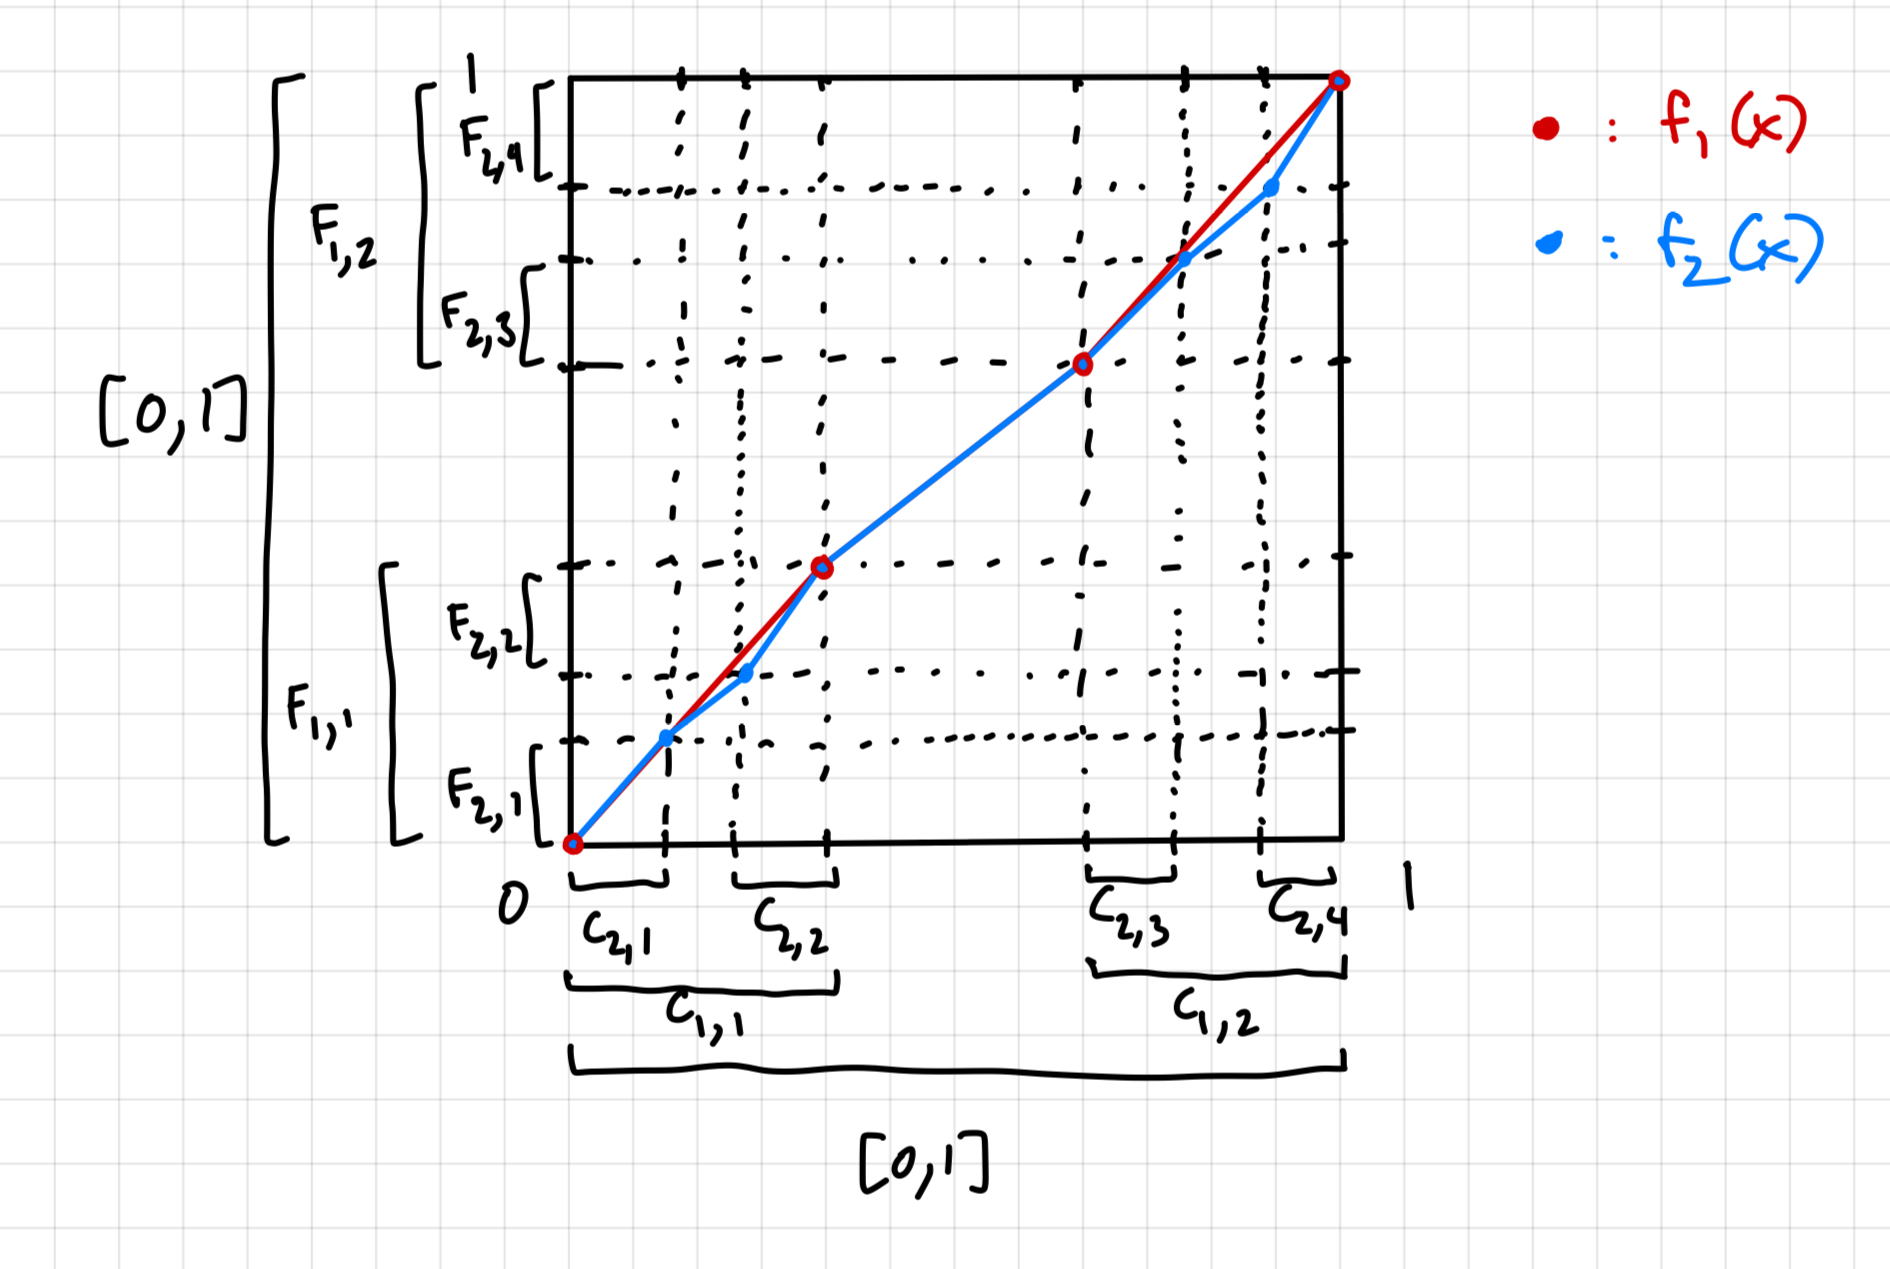
\includegraphics[width = 12cm]{figures/3.33.jpeg}
    \end{center}

    We now WTS that $\{f_n(x)\}$ uniformly converges, i.e., converges in $(C^0([0, 1]), d_{\sup})$.

    Note that for $m > n$, $f_m$ agrees with $f_n$ on $C_n^C$, so \[
        d_{\sup}(f_m, f_n) = \sup_{x \in [0, 1]} |f_m(x) - f_n(x)| = \sup_{x \in C_n} |f_m(x) - f_n(x)| \leq (3/8)^n
    \]
    Therefore, for any $\epsilon > 0$, we can choose $N$ sufficiently large such that $(3/ 8)^N < \epsilon$. Then for $m, n \geq N $ \[
        d(f_m, f_n) = \sup_{x \in [0, 1]} |f_m(x) - f_n(x)| < \epsilon
    \]
    so $\{f_n\}$ is Cauchy, and converges to some $h$. Each $f_n$ is continuous so $h$ must also be continuous. $h$ is also a bijection, and maps from [0, 1] compact to [0, 1]. It is therefore a homeomorphism.

    This $h$ maps $C$ to $F$, because $C^C$ is mapped to $F^C$. This is because
    \[
        C^C = \bigcup_{k \in \bbn} C_k^C
    \]
    and for any $k \in \bbn$, $f_l(x)$ for $l \geq k$ agree on $C_k^C$ (send to the same points in $F_k^C$). It follows that $h(x)$ also sends $C_k^C$ to $F_k^C$ (uniform convergence implies pointwise convergence). This is true for all $k \in \bbn$.

    We therefore have a homeo $h: [0, 1] \to [0, 1]$ that maps $C$ to $F$. \qed

    \textbf{(c)} It is clear that $\chi_C \circ h^{-1} = \chi_F$.

    $h^{-1}$ is a homeo on [0, 1] so it is clearly RI. From (a), $\chi_C$ is also RI, but $\chi_F$ is not.

    Corollary 28 doesn't apply here because $\chi_C$ is RI and $h^{-1}$ is continuous, not the other way around.

    Corollary 32 doesn't apply because $(h^{-1})^{-1} = h$ is not Lipschitz. It sends a zero set ($C$) to a non-zero set ($F$)
\end{solution}

\begin{problem} [IV]
This exercise is about the middle thirds Cantor set $C$.
\begin{enumerate} [(a)]
    \item Let $I_L$ be the interval [0, 1/3] and let $I_R$ be the interval [2/3, 1]. Let $C_L = C \cap I_L$ and $C_R = C \cap I_R$. Define maps $f_L: I_L \to [0, 1]$ and $f_R: I_R \to [0, 1]$ by $f_L(x) = 3x$ and $f_R(x) = 3x-2$. Prove that \[
              f_L(C_L) = f_R(C_R) = C
          \]
          How can you use these maps to systematically label points in $C$?

    \item Find 4 squares $R_1, \dots, R_4 \subset [0, 1]^2$ and 4 affine maps $f_i: R_i \to [0, 1]^2, i = 1, \dots, 4$ such that, if we set $(C \times C)_i = (C \times C) \cap R_i$, then \[
              C \times C = (C \times C)_1 \cup \dots (C \times C)_4
          \]
          and $f_i((C\times C)_i) = C \times C$. How can you use these maps to systematically label points in $C \times C$? See Figure 1.
          \begin{center}
              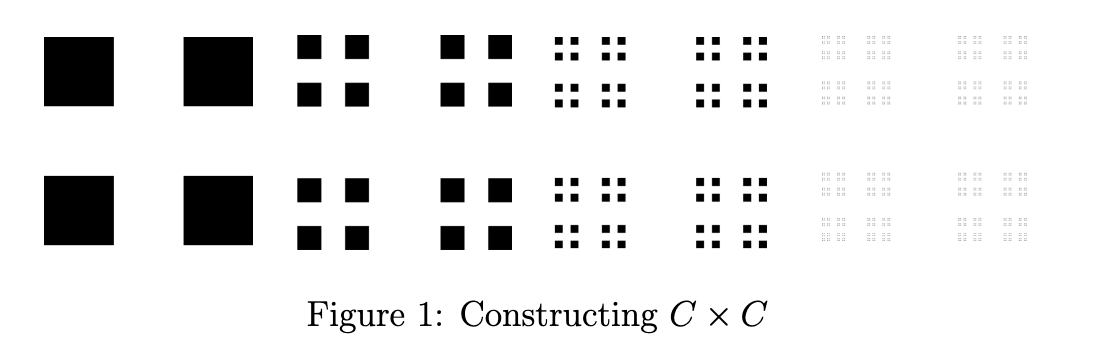
\includegraphics[width = 8cm]{./figures/cantorfigure1.png}
          \end{center}
    \item Prove that $C \times C$ is homeomorphic to $C$.
    \item Suppose you divide $[0, 1]^2$ into 9 equal smaller squares, remove the interior of the middle ninth square from $[0, 1]^2$, repeat removing the inner ninth from the remaining squares, etc., and intersect to obtain a compact set $M$. Why is $M$ not homeomorphic to $C \times C$?
    \item Prove that every real number $r \in [0, 2]$ can be written as a sum $x +y$, where $x, y \in C$. (Equivalently, $C + C = [0, 2]$). [Hint: there are two ways to do this — algebraically and geometrically. To do algebraically, think of base 3 representations of real numbers. To do geometrically, look at the images in Figure 2]
          \begin{center}
              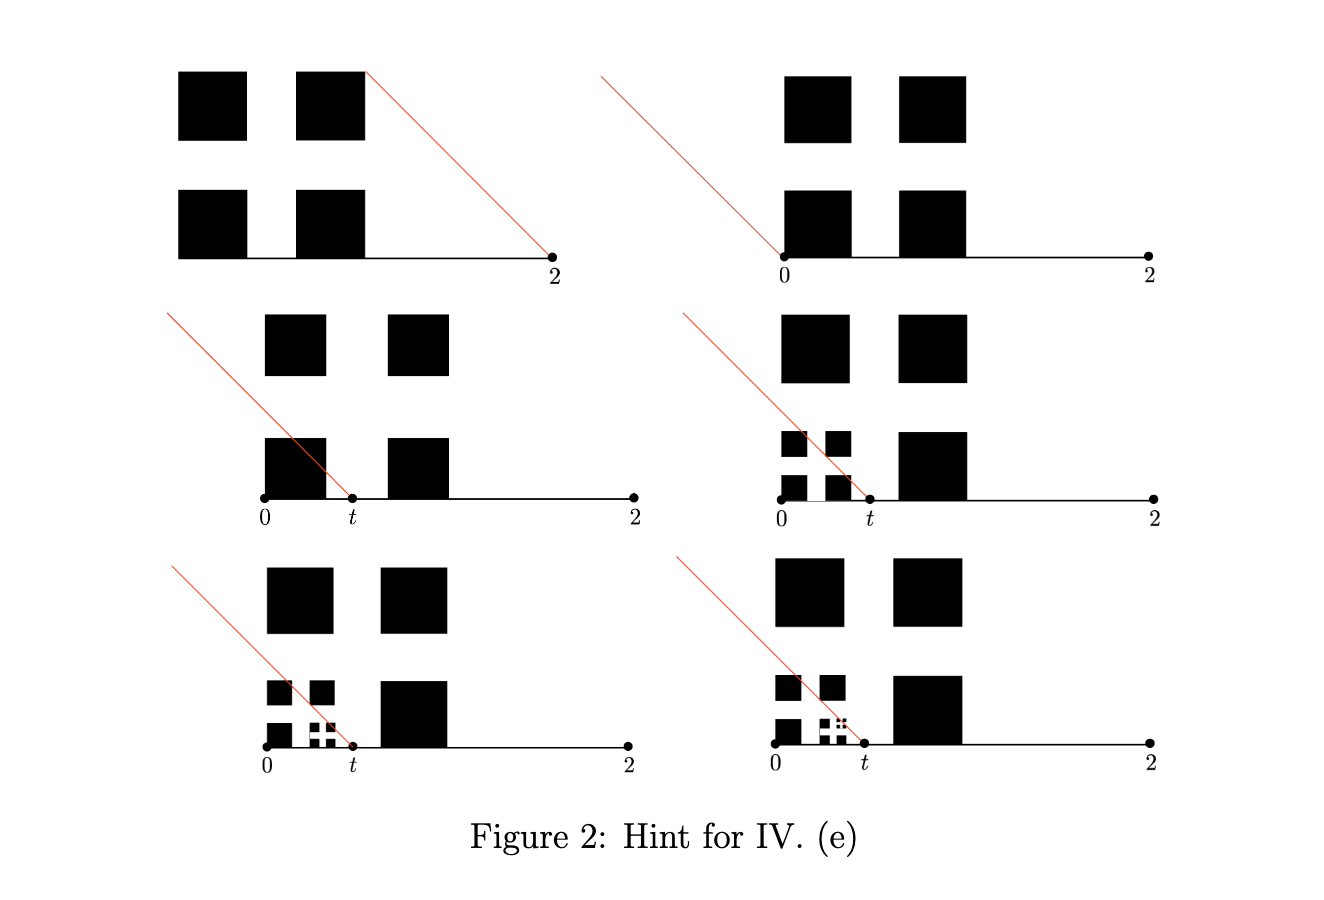
\includegraphics[width = 12cm]{./figures/cantorfigure2.png}
          \end{center}
    \item (EC) Fix $a \in [1, 3]$. For which $b$ does the equation $ax + y = b$ always have a solution with $x, y \in C$? What happens when $a > 3$?
\end{enumerate}
\end{problem}
\begin{solution}
    \textbf{(a)} WTS $f_L(C_L) = C$.

    The construction of $C$ yields an alternative expression for $C$:
    \[
        C = [0, 1]\backslash\left\{\left(\frac{3k+1}{3^m}, \frac{3k+2}{3^m}\right) \mid k, m \in \bbn\right\}
    \]
    since these are the intervals removed from $C_{m-1}$ to form $C_m$ ($C_0 \equiv [0, 1]$).

    Let $x \in C_L$. Suppose $f_L(x) = 3x \not \in C$ then \[
        3x \in \left( \frac{3k+1}{3^m}, \frac{3k+2}{3^m} \right)
    \]
    for some $k, m \in \bbn$. But this implies \[
        x \in \left( \frac{3k+1}{3^{m+1}}, \frac{3k+2}{3^{m+1}} \right)
    \]
    so $x \not \in C$, \contra

    It follows that $3x \in C$. This implies $f_L(C_L) \subseteq  C$

    Let $y \in C$, WTS $\frac{y}{3} \in C_L$. This direction is similar, so $C \subseteq f_L(C_L)$.

    It follows that $f_L(C_L) = C$.

    The proof for $f_R(C_R) = C$ is similar, since we can reflect [0, 1] and translate 1 unit in the positive $x-$direction. Then $f^{flipped}_R(x') = 3x'$. \qed


    It's trivial that $C \cap (1/3, 2/3) = \emptyset$. It follows that \[
        C  = (C \cap I_L) \sqcup (C \cap I_R)
    \]
    Given $x_0 \in C$. Label $x_0$ as an infinite string of `L' and `R' as follows:


    \begin{enumerate}
        \item Since $x_0 \in C = (C \cap I_L) \sqcup (C \cap I_R)$, we have $x_0 \in C \cap I_L$ or $x_0 \in C \cap I_R$. Initialize $x' = x_0$.
        \item If $x' \in C_L$, add to string of $x_0$ `L'. Assign $f_L(x') \to x'$.
        \item Else ($x' \in C_R$), add to string of $x_0$ `R'. Assign $f_R(x') \to x'$.
        \item Repeat (2) and (3) with new value of $x'$.
    \end{enumerate}

    \textbf{(b)} Define $R_1 \coloneqq I_L \times I_L, R_2 \coloneqq I_L \times I_R, R_3 \coloneqq I_R \times I_L, R_4 \coloneqq I_R \times I_R$ and
    \[
        \begin{aligned}
            f_1: R_1 \to [0, 1]^2 &  & (x, y) \mapsto (f_L(x), f_L(y)) \\
            f_2: R_2 \to [0, 1]^2 &  & (x, y) \mapsto (f_L(x), f_R(y)) \\
            f_3: R_3 \to [0, 1]^2 &  & (x, y) \mapsto (f_R(x), f_L(y)) \\
            f_4: R_4 \to [0, 1]^2 &  & (x, y) \mapsto (f_R(x), f_R(y))
        \end{aligned}
    \]
    Then $(C \times C)_1 = (C \times C) \cap R_1 = C_L \times C_L$. Similar for $i = 2, 3, 4$. Since $C = C_L \sqcup C_R$, it follows that \[
        C \times C = \bigcup_{i=1}^4 (C \times C)_i
    \]

    Furthermore, \[
        f_1 ((C \times C)_1) = f_1 (C_L \times C_L) = C \times C
    \]
    since $f_L(C_L)$ as proven in (a). The same proof applies for $i = 2, 3, 4$.

    We can now label $(x_0, y_0) \in C \times C$ as a infinite string of `L' and `R' as follows:
    \begin{enumerate}
        \item Initialize $x' = x_0, y' = y_0$.
        \item If $x' \in C_L$, add `L' to string. Assign $f_L(x') \to x'$.
        \item Else ($x' \in C_R$), add `R' to string. Assign $f_R(x') \to x'$.
        \item If $y' \in C_L$, add `L' to string. Assign $f_L(y') \to y'$.
        \item Else ($y' \in C_R$), add `R' to string. Assign $f_R(y') \to y'$.
        \item Repeat from (2) with new values of $x'$ and $y'$.
    \end{enumerate}

    \textbf{(c)} Construct function $h: C \times C \to C$, $(x_0, y_0) \in C \times C$ gets mapped to $z_0$ of the same L, R label sequence.

    More concretely, let $S$ be the set of all infinite sequence of `L' and `R'. Then there exists the labeling bijection as constructed in (a) $l_1: C \times S$, and the label bijection as constructed in (b) $l_2: C \times C \to S$. Then $h = l_2^{-1} \circ l_1$ is a bijection.

    By construction of $l_1$, we have \[
        l_1^{-1}(s): S \to C
    \]
    that maps \[
        s \mapsto \sum_{k \in \bbn} \frac{2}{3^k}\delta(s[k], `R')
    \]
    where $s[k]$ is the $k-$th letter of string $s$, and $\delta(s_k, `R')$ returns 1 if $s[k]$ is `R', 0 otherwise. We now endow $S$ with the metric \[
        d_S(s_1, s_2) = d_C(l_1^{-1}(s_1), l_1^{-1}(s_2))
    \]

    Given $s_0 \in S, \epsilon > 0$, then there exists $N \in \bbn$ such that $1/3^N < \epsilon$.

    Let $x_0 = l_1^{-1}(s_0)$. Then for any $x' \in B_C(x_0, 1/3^N), s' = l_1(x') = `s_0[1]s_0[2]\dots s_0[N]\dots'$

    This is because $d_C(x', x_0) < 1/3^N$ so \[
        |\sum_{k \in \bbn} \frac{2}{3^k}\delta(s'[k], 'R') - \sum_{k \in \bbn} \frac{2}{3^k}\delta(s_0[k], 'R')| < 1/3^N
    \]

    which forces $s'$ to agree with $s_0$ for the first $N$ letters.

    It follows that $d_S(s_0, l_1(x')) < 1/3^N < \epsilon$. Thus, $x' \in B_C(x_0, 1/3^N) \implies d_S(s_0, l_1(x')) < \epsilon$.

    $l_1$ is therefore continuous. $C$ is also compact. So $l_1$ is homeo.

    A similar proof for $l_2$ applies. It follows that $h$ is also a homeo. \qed

    \textbf{(d)} In short, $M$ is connected, but $C \times C$ is disconnected, so they can't be homeomorphic.

    % We want to show that $M$ is connected. Let $M_1$ be $[0, 1]^2 \backslash [1/3, 2/3]^2$ and so on. Then \[
    % M = \bigcap_{n \in \bbn}{M_n}
    % \]
    % Suppose $M$ is disconnected, then there exists a proper clopen subset $A$ of $M$, which implies $A \$
    \qed

    \textbf{(e)} Rephrasing the question, we want to show that the line \[
        l: x + y = r
    \]
    satisfies $l \cap (C \times C) \neq \emptyset$ for all $r \in [0, 2]$.

    \textbf{Case 1:} $r \in C$.

    Then there is a trivial intersection $(r, 0) \in l \cap C \times C $.

    \textbf{Case 2:} $r \not \in C$.

    Then $r$ was in the middle third of some subinterval $C_{N, k} \subseteq C_N$. Call the thirds of $C_{N, K} = I_L \sqcup I_M \sqcup I_R$, then $r \in I_M$. Note that the length of $I_L, I_M, I_R$ is $1/3^N$. For convenience, let $q = 1/3^N$.

    We now WTS that $l \cap (I_L \times [0, 1/3^N]) \neq \emptyset$.

    Denote $I_L = [a, a + q], I_M = (a + q, a + 2q), I_R = [a + 2q, a + 3q]$ then $r = a + q + p$ where $p \in (0, q)$.

    Then $a + q \in I_L, p \in (0, q) \subset [0, 1/3^N] \implies \:\text{Point}\:  (a + q, p) \in (I_L \times [0, 1/3^N])$. Furthermore, $(a + q) + p = r$ trivially, so point $(a + q, p) \in l$.

    Thus, $l \cap (I_L \times [0, 1/3^N]) \neq \emptyset$. And $(I_L \times [0, 1/3^N]) \subset (C_N \times C_N) \implies l \cap (C_N \times C_N) \neq \emptyset$.

    An easy consequence of this is that since $C_N \subset C_n \forall n \leq N \implies l \cap (C_n \times C_n) \neq \emptyset \forall n \leq N$.

    We want to show that $l \cap (C_{N+1} \times C_{N+1}) \neq \emptyset$. Since $l \cap (C_N \times C_N) \neq \emptyset$, \[
        l \cap (I_x \times I_y) \neq \emptyset
    \]
    where $I_x, I_y \subset C_N$, are some of the $2^N$ intervals that make up $C_N$.

    The follow pictorial proof (which can easily be rigorized) shows that $l$ must lie in 1 of 3 zones of $I_x \times I_y$ divided by the blue lines, and therefore intersect one of the ``corner squares''. It follows that $l \cap (C_{N+1} \times C_{N+1}) \neq \emptyset$.
    \begin{center}
        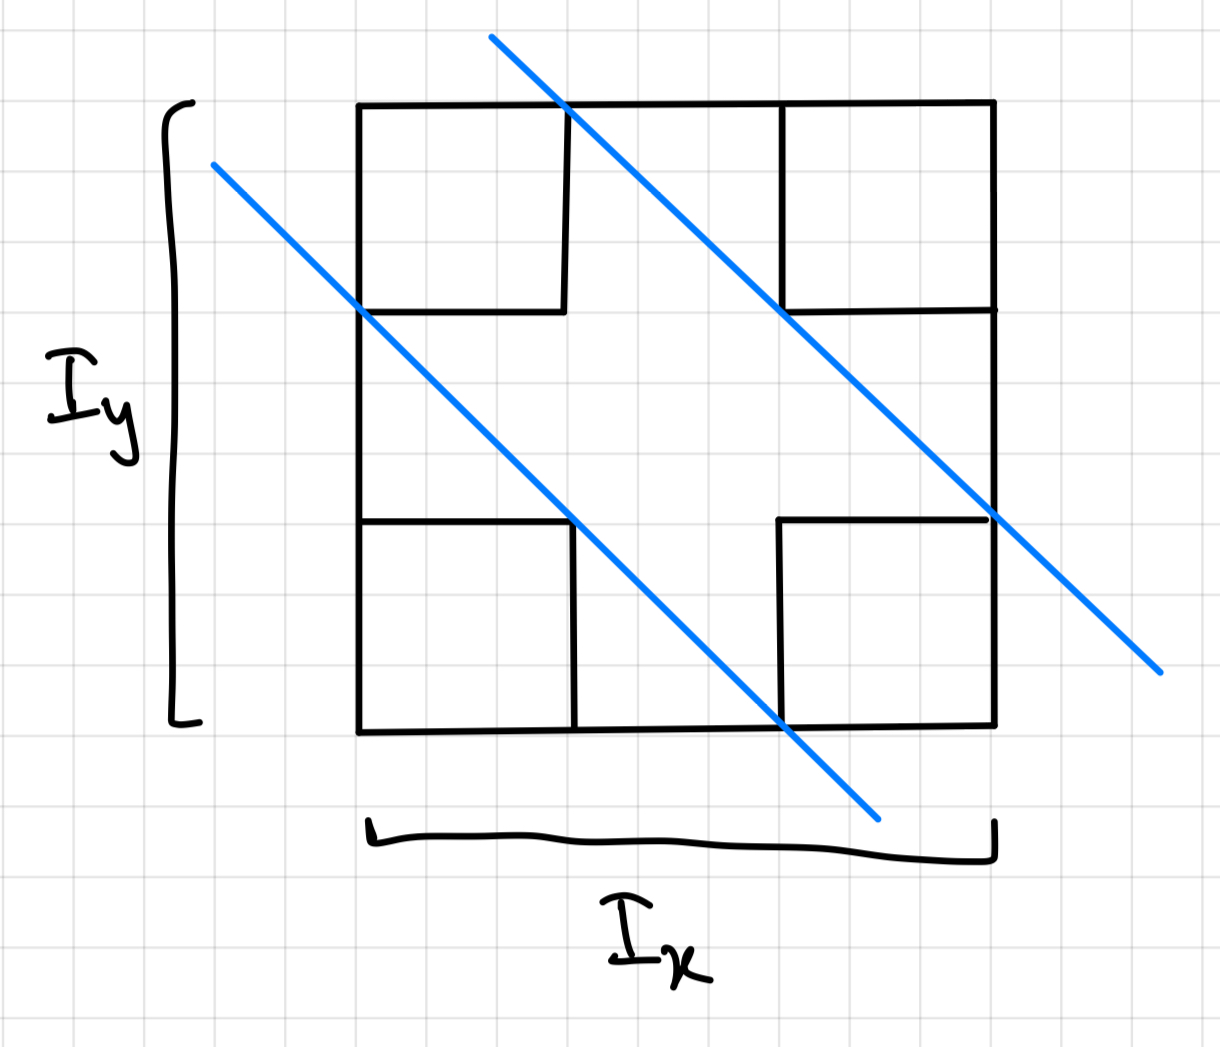
\includegraphics[width=6cm]{./figures/cantorfigure3.jpeg}
    \end{center}

    By induction, it follows that $l \cap (C_n \times C_n) \forall n \geq N$.

    Combining the 2 subparts, it follows that $l \cap (C_n \times C_n) \forall n \in \bbn \implies l \cap (C \times C)$.
\end{solution}
\end{document}